\documentclass[13pt, a4paper, twoside]{mwart}
\usepackage[a4paper]{geometry}
\geometry{left=3cm}
\geometry{right=1.5cm}
\geometry{top=2cm}
\geometry{bottom=1.5cm}
\usepackage[pdftex]{graphicx}
\usepackage{float}
\graphicspath{{img/}}

\usepackage[utf8]{inputenc}
\usepackage{polski}
\usepackage[polish]{babel}
\usepackage{tabularx}
\usepackage{datetime}
\usepackage{listings}
\lstset{basicstyle=\footnotesize}

\newcommand{\coursename}{Modelowanie i Analiza Systemów}
\newcommand{\labnumber}{4}
\newcommand{\labname}{Model idealnego przetwornika A/C typu Sigma--Delta}
\newcommand{\studentname}{Maciej Stanek}
\newcommand{\studentnumber}{122352}
\newdate{labdate}{17}{5}{2018}
\newdate{labreportdate}{3}{6}{2018}

\usepackage{fancyhdr}
\pagestyle{fancy}
\fancyhead[RO,LE]{\thepage}
\fancyhead[LO]{\textbf{LAB\#\labnumber} \labname}
\fancyhead[RE]{\coursename}
\fancyfoot{}

\usepackage{xcolor}
\usepackage{framed}
\colorlet{shadecolor}{gray!10}
\newcounter{taskcounter}
\newcommand{\task}[1]{
  \stepcounter{taskcounter}
  \vspace{0.2cm}
  \begin{shaded}
    \noindent\textbf{Zadanie \thetaskcounter:} \textit{#1}%
  \end{shaded}
  \vspace{0.2cm}}

\renewcommand{\labelitemi}{$\bullet$}

\begin{document}

\begin{center}
  \textbf{\LARGE{Sprawozdanie z laboratorium}}
\end{center}

\noindent
\begin{tabularx}{\linewidth}{rX}
  \textbf{Przedmiot} & \coursename \\
  \textbf{Temat laboratorium} & \labname \\
  \textbf{Numer laboratorium} & \labnumber \\
  \textbf{Imię i nazwisko} & \studentname \\
  \textbf{Numer indeksu} & \studentnumber \\
  \textbf{Data wykonania} & \displaydate{labdate} \\
  \textbf{Data sprawozdania} & \displaydate{labreportdate} \\
\end{tabularx}

\vspace{0.3cm}
\noindent\hrulefill

%%%%%%%%%%%%%%%%%%%%%%%%%%%%%%%%%%%%%%%%%%%%%%%%%%%%%%%%%%%%%%%%%%%%%%%%%%%%%%%

\task{Zaprojektuj i zaimplementuj w VHDL--AMS modele idealnych przetworników sigma--delta I i II rzędu. Do wyjścia modulatora podłącz model filtru decymacyjnego, który został opracowany w poprzednich zadaniach. Elementy układu (entity) powinny mieć porty typu \texttt{terminal}. Integratory zaimplementuj wykorzystując opis w dziedzinie Z.}

Zgodnie z zaleceniem prowadzącego, implementacji modulatora dokonano w dziedzinie ciągłej. Wymagało to przygotowania układu całkującego działającego na obiektach typu \texttt{terminal}.

\lstinputlisting[
  language=VHDL,
  caption={Układ całkujący.}
  ]{../122352/hdl/analog_int.vhd}

\begin{figure}[H]
	\centering
  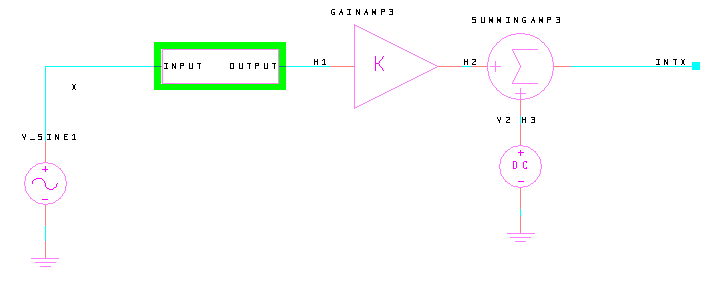
\includegraphics[width=0.6\linewidth]{inv/x_intx_sch.png}
  \caption{Układ testujący moduł całkujący.}
\end{figure}

\begin{figure}[H]
	\centering
  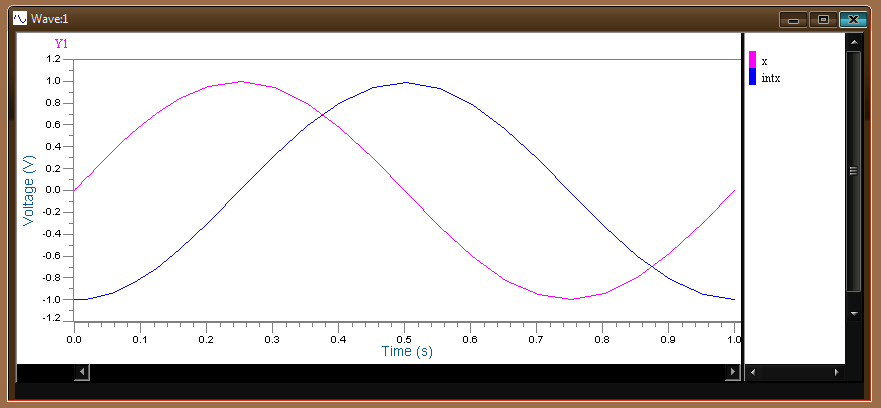
\includegraphics[width=0.6\linewidth]{inv/x_intx.png}
  \caption{Test modułu całkującego.}
\end{figure}

Następnie wykonano modulatory w dwóch żądanych konfiguracjach. Wymagało to modyfikacji kodu decymatora, którzy został przygotowany na minionych zajęciach.

\begin{figure}[H]
	\centering
  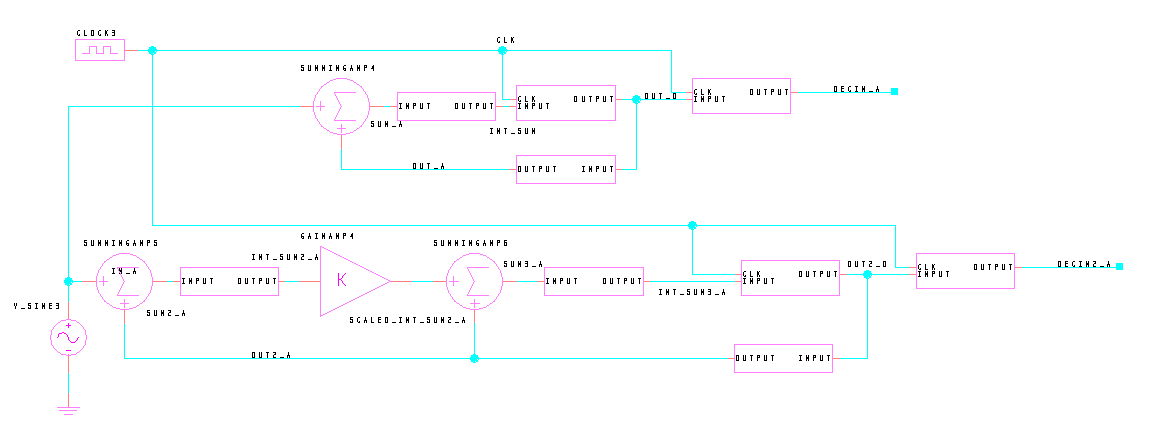
\includegraphics[width=0.9\linewidth]{inv/sigma_delta_2_sch.png}
  \caption{Modulatory sigma--delta z dołączonymi decymatorami. Od góry kolejno układy pierwszego i drugiego rzędu.}
\end{figure}

\lstinputlisting[
  language=VHDL,
  caption={Układ decymacyjny: zmodyfikowany kod źródłowy.}
  ]{../122352/hdl/decim.vhd}

\begin{figure}[H]
	\centering
  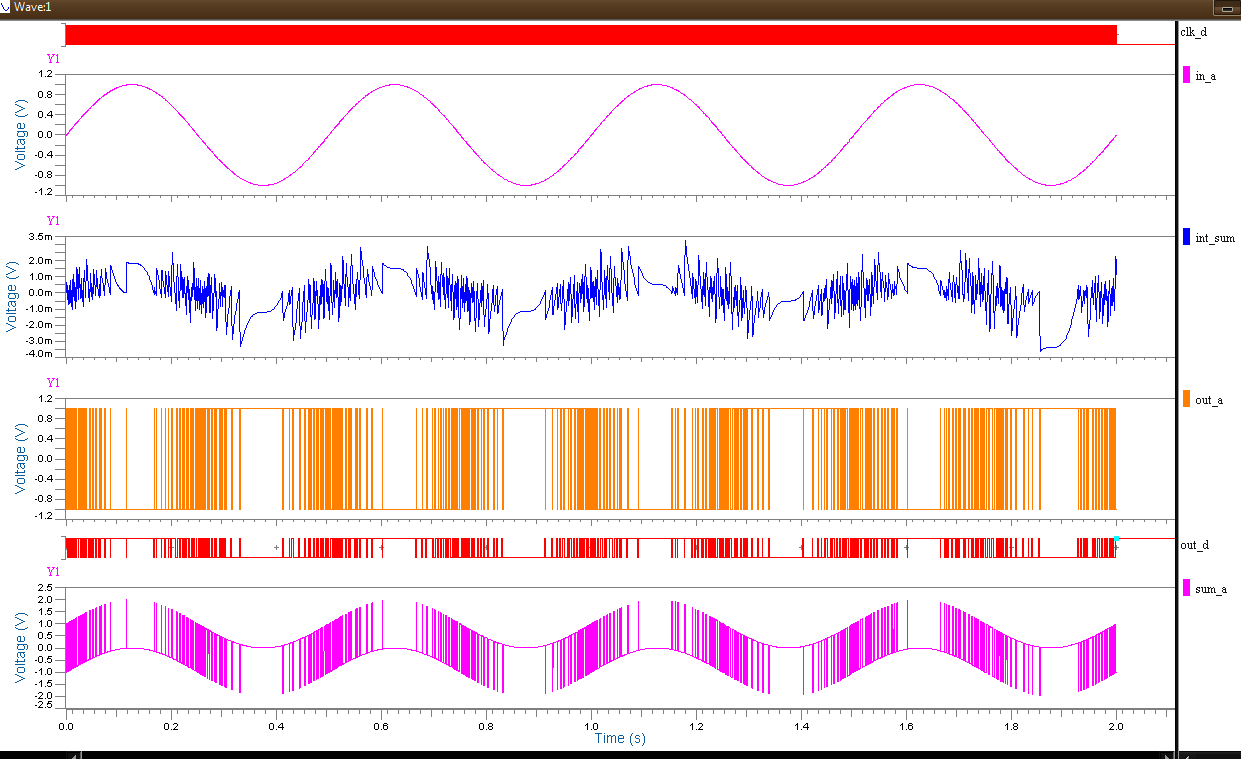
\includegraphics[width=\linewidth]{inv/sigma_delta.png}
  \caption{Działanie modulatora sigma--delta pierwszego rzędu. Sygnał \texttt{out\_d} to sygnał wyjściowy modulatora.}
\end{figure}

\begin{figure}[H]
	\centering
  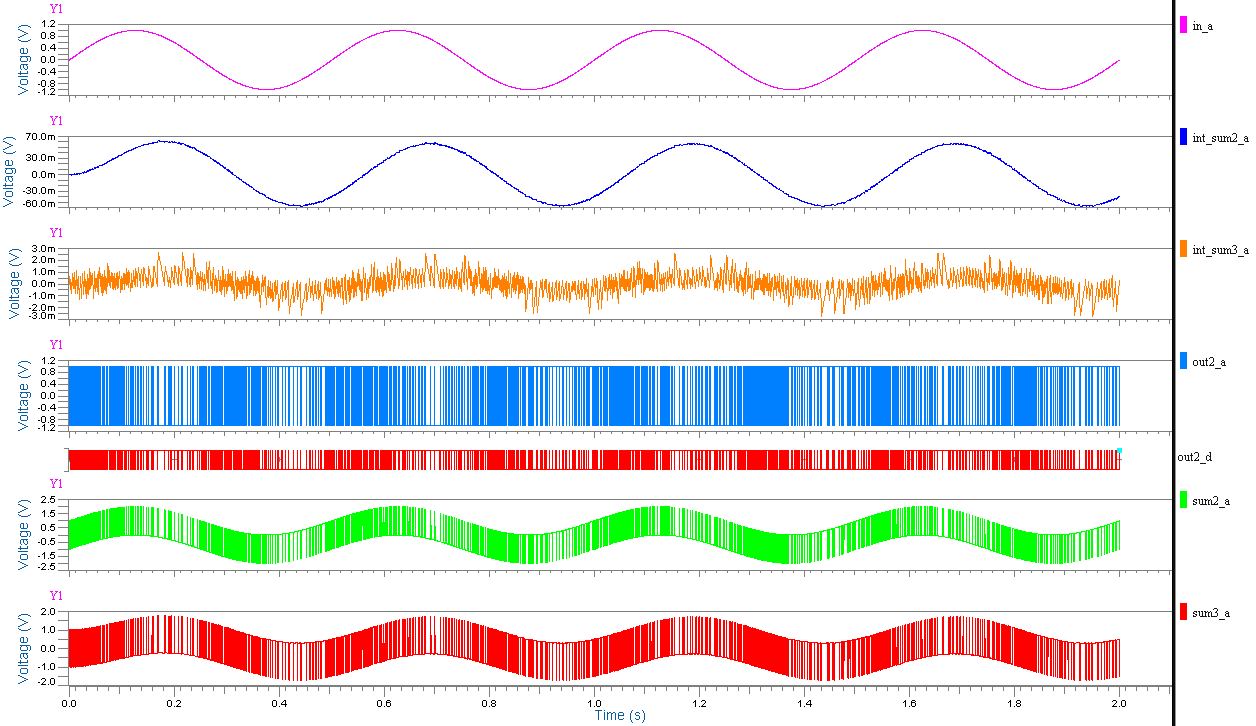
\includegraphics[width=\linewidth]{inv/sigma_delta_2.png}
  \caption{Działanie modulatora sigma--delta drugiego rzędu. Sygnał \texttt{out2\_d} to sygnał wyjściowy modulatora.}
\end{figure}

\begin{figure}[H]
	\centering
  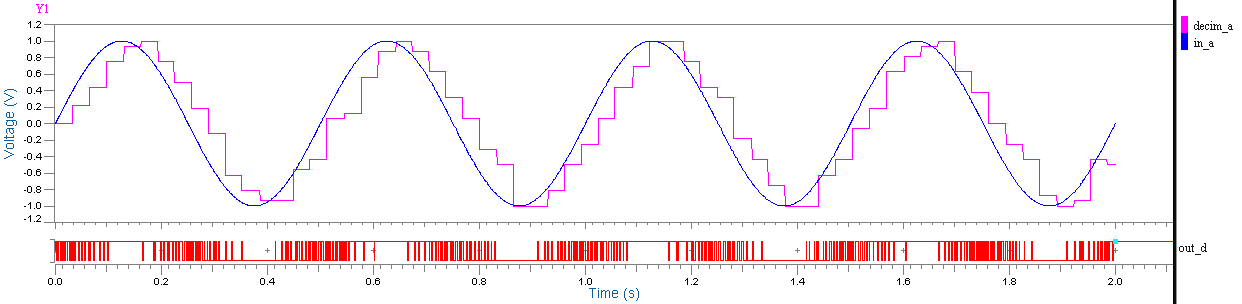
\includegraphics[width=0.9\linewidth]{inv/sigma_delta_decymator.png}
  \caption{Sygnał przetworzony w modulatorze pierwszego rzędu i odtworzony układem decymacyjnym. Współczynnik OSR wynosi domyślne 32.}
\end{figure}

\begin{figure}[H]
	\centering
  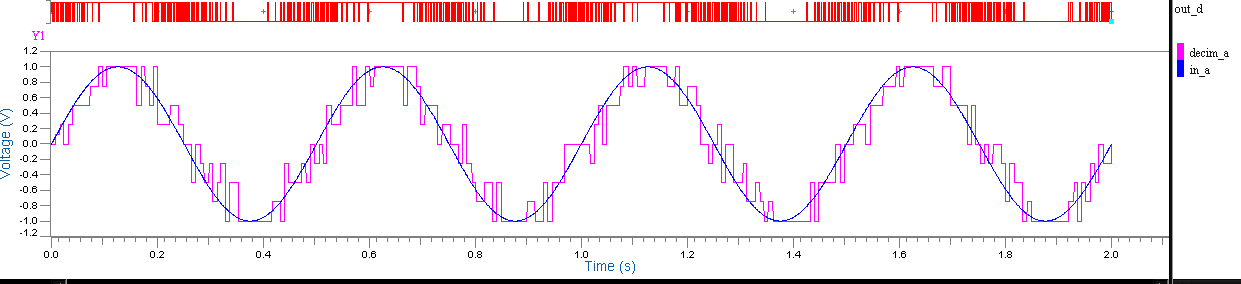
\includegraphics[width=0.9\linewidth]{inv/sigma_delta_decymator_osr8.png}
  \caption{Sygnał przetworzony w modulatorze pierwszego rzędu i odtworzony układem decymacyjnym. Współczynnik OSR wynosi 8.}
\end{figure}

\begin{figure}[H]
	\centering
  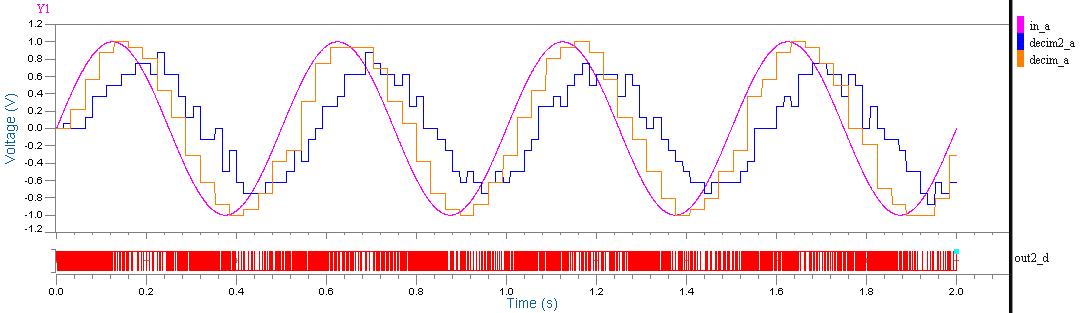
\includegraphics[width=0.9\linewidth]{inv/sigma_delta_2_rzedu_porownanie.png}
  \caption{Sygnał przetworzony w modulatorze drugiego rzędu i odtworzony układem decymacyjnym (niebieski) porównany z sygnałem przetworzonym przez modulator pierwszego rzędu (pomarańczowy). Współczynnik OSR dla obydwu konfiguracji wynosi domyślne 32.}
\end{figure}

%%%%%%%%%%%%%%%%%%%%%%%%%%%%%%%%%%%%%%%%%%%%%%%%%%%%%%%%%%%%%%%%%%%%%%%%%%%%%%%

\end{document}
